\documentclass[11pt, a4paper,english,spanish]{article}
\usepackage[spanish]{babel}
\usepackage[utf8]{inputenc}
\parskip = 11 pt
\usepackage[width=18cm, left=1.5cm, top=2.25cm, height= 25cm]{geometry}

\usepackage{amsmath}
\usepackage{algorithm}
\usepackage[noend]{algpseudocode}
\usepackage{amsfonts}
\usepackage{amssymb}
\usepackage{fancyhdr}
\usepackage{lastpage}
\usepackage{caratula}
\usepackage{url}
\usepackage{flafter}
\usepackage{afterpage}
\usepackage{float}
\usepackage{listings}
\usepackage{color}
\usepackage{verbatim}
\usepackage{placeins}
\usepackage{graphicx}
\usepackage{caption}
\usepackage{subcaption}

\usepackage{titlesec}
\usepackage{hyperref}

\titleclass{\subsubsubsection}{straight}[\subsection]

\newcounter{subsubsubsection}[subsubsection]
\renewcommand\thesubsubsubsection{\thesubsubsection.\arabic{subsubsubsection}}
\renewcommand\theparagraph{\thesubsubsubsection.\arabic{paragraph}} % optional; useful if paragraphs are to be numbered

\titleformat{\subsubsubsection}
  {\normalfont\normalsize\bfseries}{\thesubsubsubsection}{1em}{}
\titlespacing*{\subsubsubsection}
{0pt}{3.25ex plus 1ex minus .2ex}{1.5ex plus .2ex}

\makeatletter
\renewcommand\paragraph{\@startsection{paragraph}{5}{\z@}%
  {3.25ex \@plus1ex \@minus.2ex}%
  {-1em}%
  {\normalfont\normalsize\bfseries}}
\renewcommand\subparagraph{\@startsection{subparagraph}{6}{\parindent}%
  {3.25ex \@plus1ex \@minus .2ex}%
  {-1em}%
  {\normalfont\normalsize\bfseries}}
\def\toclevel@subsubsubsection{4}
\def\toclevel@paragraph{5}
\def\toclevel@paragraph{6}
\def\l@subsubsubsection{\@dottedtocline{4}{7em}{4em}}
\def\l@paragraph{\@dottedtocline{5}{10em}{5em}}
\def\l@subparagraph{\@dottedtocline{6}{14em}{6em}}
\makeatother

\setcounter{secnumdepth}{4}
\setcounter{tocdepth}{4}
\definecolor{gray97}{gray}{.97}
\definecolor{gray75}{gray}{.75}
\definecolor{gray45}{gray}{.45}

\algdef{SE}[DOWHILE]{Do}{doWhile}{\algorithmicdo}[1]{\algorithmicwhile\ #1}%

\usepackage{listings}
\lstset{ frame=Ltb,
     framerule=0pt,
     aboveskip=0.5cm,
     framextopmargin=3pt,
     framexbottommargin=3pt,
     framexleftmargin=0.4cm,
     framesep=0pt,
     rulesep=.4pt,
     backgroundcolor=\color{gray97},
     rulesepcolor=\color{black},
     %
     stringstyle=\ttfamily,
     showstringspaces = false,
     basicstyle=\small\ttfamily,
     commentstyle=\color{gray45},
     keywordstyle=\bfseries,
     %
     numbers=left,
     numbersep=15pt,
     numberstyle=\tiny,
     numberfirstline = false,
     breaklines=true,
   }


% minimizar fragmentado de listados
\lstnewenvironment{listing}[1][]
   {\lstset{#1}\pagebreak[0]}{\pagebreak[0]}
 
\lstdefinestyle{consola}
   {basicstyle=\scriptsize\bf\ttfamily,
    backgroundcolor=\color{gray75},
   }
 
\lstdefinestyle{C++}
   {language=C++,
   }
 
\newcommand{\real}{\ensuremath{\mathbb{R}}}
\newcommand{\grad}{\hspace{-2mm}$\phantom{a}^{\circ}$}

\pagestyle{fancy}

\title{MotionCapture}

%Estilo para el encabezado
\fancyhead[LO, LE]{Métodos Numéricos}
\fancyhead[RO, RE]{2$^{do.}$ cuatrimestre de 2014}
\fancyhead[CO, CE]{}

\fancyfoot[CO, CE]{P\'agina \thepage\ de \pageref{LastPage}}

\begin{document}
%Estos son los parametros para la caratula
\materia{Métodos Numéricos}
\submateria{Trabajo Pr\'actico Nro. 3}
\titulo{Demosaicing}
\fecha{\today}
\integrante{Martin Carreiro}{45/10}{martin301290@gmail.com}
\integrante{Kevin Kujawski}{459/10}{kevinkuja@gmail.com}
\integrante{Juan Manuel Ort\'iz de Z\'arate}{403/10}{jmanuoz@gmail.com}
\maketitle
\newpage

%Pagina de titulo e indice
\thispagestyle{empty}

\tableofcontents

%\newpage

\normalsize
\section{Resumen}
En el siguiente trabajo investigaremos el comportamiento de distintos algoritmos pensados para resolver el problema de Demosaicing. Describiremos sus distintos funcionamientos, 
realizaremos pruebas transversales a todos ellos y pruebas particualres a cada uno. Con el objetivo de, en primera instancia, hacer comparaciones a grandes rasgos de los resultados obtenidos para luego con 
las pruebas individuales evaluar el resultado en los casos potencialmente conflictivos de cada uno y así tener un panaroma más completo a la hora de concluir cual es el mejor o si sus eficiencias varian según
los contextos de uso.

\newpage
\section{Introducci\'on te\'orica}

El problema de Demosaicing consta de poder construir una imagen con información de los 3 canales en cada uno de sus pixel en base a una que sólo tiene definidos los valores de un sólo canal para cada celda. Este desafío es muy común en las camáras de fotos digitales ya que en realidad cada fotosensor detecta un sólo color, por lo cual a la imagen capturada hay que aplicarle algún procedimiento lógico para que el usuario final pueda verla efectivamente con todos los colores.

Particularmente estaremos analizando 4 algoritmos distintos que intentan solucionar esto. Ellos son: Vecinos, Bilineal, Direccional y High Quality. Todos estos deben aplicarse sobre imágenes en formato Bayer array, es decir, imágenes que en cada pixel tienen información sólo de un canal (Verde, Rojo o Azul) y estos además tienen una distribución especial (en la que por ejemplo el verde predomina en cantidad ya que es el color que mejor recepción tiene en el ojo humano).

Para nuestras pruebas lo que haremos es tomar imágenes con todos sus canales completos en todos lo pixeles y pasarlas al formato Bayer array. Como en lo que queremos hacer foco en este trabajo es la calidad de estos procedimientos y sus resultados, no nos interesa que la imagen Bayer haya sido tomada realmente por una cámara, es más, nos sirve más tener una imagen full color y transformala ya que así podemos comparar nuestros resultados contra la original.

Por esto es que desarrollamos una función muy simple que realiza esta transformación. Básicamente lo que hace es: 
\begin{itemize}
\item Celdas en columnas y filas pares, deja sólo el canal azul
\item Celdas en columnas y filas impares, deja sólo el canal rojo
\item En todas las otras dejamos sólo el canal verde
\end{itemize}   


\begin{figure}[h]
       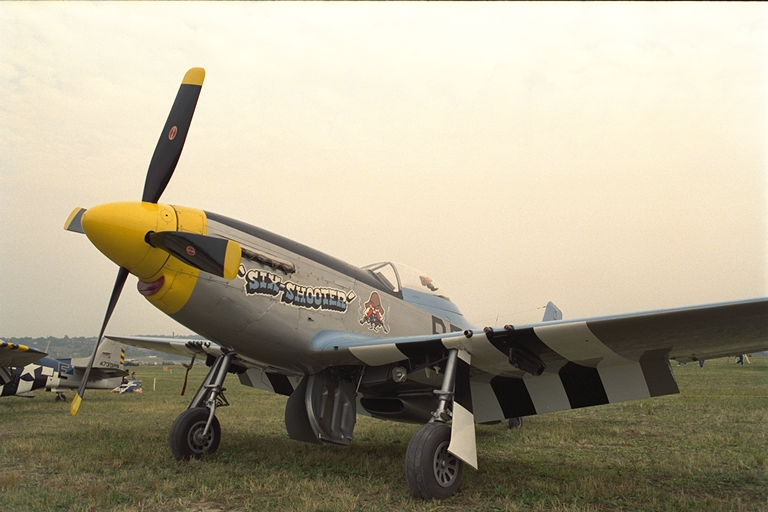
\includegraphics[width=0.5\textwidth]{imagenes/img9.png}
           \hfill
        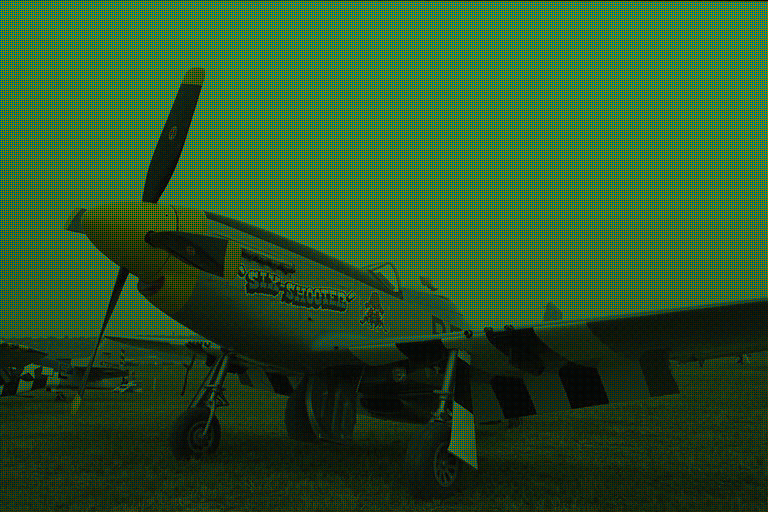
\includegraphics[width=0.5\textwidth]{imagenes/img9_bayer.png}   
        Imagen original y bayerizada
\end{figure}

\subsection{Artifacts}
\newpage
\section{Desarrollo}

Como explicamos en la introducción estaremos analizando 4 algoritmos distintos, estos son: Vecinos, Bilineal, Direccional y High Quality. En lineas generales anticiparemos que los primeros dos se utilizan para rearmar toda la imagen desde la bayerización. El resto serán utilizados para aproximar mejor el valor del verde original en los píxeles que en la bayerizción solo habían atrapado rojo y azul. Esto es porque el verde es el color que más ve el ser humano y mientras mejor esté la imagen en ese color, subjetivamente quedará mejor.\\
La idea será comparar sus resultados subjetivamente, es decir a simple vista como 
vemos la imagen resultante, objetivamente y temporalmente, cuanto tiempo demora en ejecutarse el procedimiento, para poder concluir finalmente las ventajas y desventajas de cada uno. A continuación explicaremos como 
implementamos cada uno.


\subsection{Vecinos}
Este es el más simple de todos. La idea es estabelecer el valor de los colores faltantes de cada pixel en base al vecino que tenga dicho valor. Por ejemplo si estamos en un pixel azul le preguntamos a algun vecino rojo y 
otro verde su valor y los seteamos en los correspondientes colores de nuestro pixel.

\begin{algorithm}
\caption{vecinos($imagenBayerizada$)}\label{euclid}
\begin{algorithmic}[1]
\For{$cada\ celda\ en\ imagenBayerizada$}
  \If{$celda\ es\ roja$} \Comment{Fila y columna impar}
      \State $\textit{celda.verde = vecinoIzq.verde;}$
      \State $\textit{celda.azul  = vecinoSuperiorIzq.azul;}$
  \EndIf
  \If{$celda\ es\ azul$} \Comment{Fila y columna par}
      \State $\textit{celda.rojo = vecinoInferiorDerecho.rojo;}$
      \State $\textit{celda.verde = vecinoDerecho.verde;}$
  \EndIf
  \If{$celda\ es\ verde \And fila par $}
      \State $\textit{celda.rojo = vecinoDerecho.rojo;}$ 
      \State $\textit{celda.azul = vecinoSuperior.azul;}$ 
  \EndIf
  \If{$celda\ es\ verde \And fila impar $}
      \State $\textit{celda.rojo = vecinoInferior.rojo;}$ 
      \State $\textit{celda.azul = vecinoIzquierdo.azul;}$ 
  \EndIf
\EndFor
\end{algorithmic}
\end{algorithm}

% \begin{lstlisting}[frame=single] 
% Para cada celda:
	% si es roja:
		% celda.verde = vecinoIzq.verde
		% celda.azul  = vecinoSuperiorIzq.azul	
	% si es azul:
		% celda.rojo = vecinoInferiorDerecho.rojo
		% celda.verde = vecinoDerecho.verde
	% si es verde y fila par:
		% celda.rojo = vecinoDerecho.rojo
		% celda.azul = vecinoSuperior.azul
	% si es verde y fila impar
		% celda.rojo = vecinoInferior.rojo
		% celda.azul = vecinoIzquierdo.azul
% \end{lstlisting}

Se diferencia entre fila par e impar cuando la celda es verde ya que es distinta la disposición de sus vecinos en cada caso, esto en cambio se mantiene inmutable en los casos de celda roja o azul. La selección del
vecino izquierdo y superior izquierdo cuando es roja es porque siempre existe ese vecino, a diferencia del derecho por ejemplo ya que el rojo puede ser una celda borde y no tener dicho adyacente. La misma idea aplicamos 
al caso de la celda azul y de las verdes, apuntamos a elegir el vecino que siempre existe.

\subsection{Bilineal}

La interpolación es una forma de aproximar valores desconocidos en algún punto a partir de valores que sí conocemos, sabiendo de antemano que van a tener un cierto grado de error. Esto se puede trasladar a nuestro problema, ya que tenemos que aproximar valores para un color de pixel a partir de valores cercanos conocidos, con la única diferencia que en vez de ser en una dimensión como si fuese una funcion, esta será en dos dimensiones, de ahí el nombre de $'bilineal'$. Esta interpolación en 2 dimensiones se realiza a partir de los 4 puntos más cercanos del color del pixel que queremos aproximar. Para calcular el valor de dicho punto primero se saca el promedio de los valores en dirección horizontal, luego en dirección vertical y por último el promedio de dichos valores. Cabe aclarar que dependiendo el color de pixel actual y el color que se quiera aproximar, podemos llegar a tener información de solo 2 puntos cercanos, pero alineados en la misma dirección, con lo que solo se calculará la aproximación en esa dirección.


\begin{algorithm}
\caption{bilineal($imagenBayerizada$)}\label{euclid}
\begin{algorithmic}[1]
\For{$cada\ celda\ en\ imagenBayerizada$}
  \If{$celda\ es\ roja$} \Comment{Fila y columna impar}
      \State $\textit{celda.azul = funcionLineal(puntosOblicuosALaCelda,imagenBayerizada,AZUL);}$
      \State $\textit{celda.verde = funcionLineal(puntosAdyacentesALaCelda,imagenBayerizada,VERDE);}$
  \EndIf
  \If{$celda\ es\ azul$} \Comment{Fila y columna par}
      \State $\textit{celda.rojo = funcionLineal(puntosOblicuosALaCelda,imagenBayerizada,ROJO);}$
      \State $\textit{celda.verde = funcionLineal(puntosAdyacentesALaCelda,imagenBayerizada,VERDE);}$
  \EndIf
  \If{$celda\ es\ verde \And fila par $}
      \State $\textit{celda.rojo = funcionLineal(puntosSuperiorEInferior,imagenBayerizada,ROJO);}$ 
      \State $\textit{celda.azul = funcionLineal(puntosDerechaEIzquierda,imagenBayerizada,AZUL);}$ 
  \EndIf
  \If{$celda\ es\ verde \And fila impar $}
      \State $\textit{celda.azul = funcionLineal(puntosSuperiorEInferior,imagenBayerizada,AZUL);}$ 
      \State $\textit{celda.rojo = funcionLineal(puntosDerechaEIzquierda,imagenBayerizada,ROJO);}$ 
  \EndIf
\EndFor
\end{algorithmic}
\end{algorithm}

\begin{algorithm}
\caption{funcionLineal($puntos,imagenBayerizada,color$)}\label{euclid}
\begin{algorithmic}[1]
\State $\textit{resultado $=$ 0;}$
\State $\textit{cantPuntos $=$ 0;}$
\For{$cada\ punto\ en\ puntos$}
  \If{$punto\ enRango$}
      \State $\textit{resultado $+=$ punto.color}$
      \State $\textit{cantPuntos $+=$ 1}$
  \EndIf
\EndFor
\Return $resultado/cantPuntos$
\end{algorithmic}
\end{algorithm}

% \begin{verbatim}
% Para todos los pixeles de la imágen:
%   Si estoy parado en un pixel azul:
%     Calculo el valor de rojo que tendrá el pixel 
%     haciendo el promedio de los valores en rojo de los 
%     4 puntos oblicuos a este (que estén en rango).
    
%     Calculo el valor de verde que tendrá el pixel 
%     haciendo el promedio de los valores en verde de los 

%     4 puntos adyacentes a este (que estén en rango).
%   Si estoy parado en un pixel rojo:
%     Calculo el valor de azul que tendrá el pixel 
%     haciendo el promedio de los valores en azul de los 
%     4 puntos oblicuos a este (que estén en rango).
    
%     Calculo el valor de verde que tendrá el pixel 
%     haciendo el promedio de los valores en verde de los 
%     4 puntos adyacentes a este (que estén en rango).

%   Si estoy parado en un pixel verde:
%     Si estoy parado en una fila de azules:
%       Calculo el valor de rojo que tendrá el pixel 
%       haciendo el promedio de los valores en rojo de los 
%       2 puntos superiores e inferiores (que estén en rango).

%       Calculo el valor de azul que tendrá el pixel 
%       haciendo el promedio de los valores en azul de los 
%       2 puntos a derecha e izquierda (que estén en rango).

%     Si estoy parado en una fila de rojos:
%       Calculo el valor de azul que tendrá el pixel 
%       haciendo el promedio de los valores en azul de los 
%       2 puntos superiores e inferiores (que estén en rango).

%       Calculo el valor de rojo que tendrá el pixel 
%       haciendo el promedio de los valores en rojo de los 
%       2 puntos a derecha e izquierda (que estén en rango).  
% \end{verbatim}

\newpage
\subsection{Direccional}

Para este algoritmo nos basamos en lo explicado por Burden y Faires$[1]$ para el cálculo de los splines y en lo desarrollado por Ron Kimmel$[2]$ para el algoritmo en sí. El método lo aplicamos sólo para el color verde mientras que para los otros utilizamos bilineal. 

\begin{algorithm}
\caption{direccional($imagenBayerizada$)}\label{euclid}
\begin{algorithmic}[1]
\State $\textit{hacerBilineal(imagenBayerizada)}$
\State $\textit{coeficientes $=$ new Matrix([0,0])}$ \Comment De la tupla el primero representa el coeficiente horizonal, el otro el vertical
\For{$cada\ fila\ en\ imagenBayerizada.menosPrimerayUltima$}
  \State $resolverPorSpline(horizontal,fila)$ \Comment Llenará la matriz de coeficientes
\EndFor
\For{$cada\ columna\ en\ imagenBayerizada.menosPrimerayUltima$}
  \State $resolverPorSpline(vertical,columna)$ \Comment Llenará la matriz de coeficientes
\EndFor
\For{$cada\ celda\ en\ imagenBayerizada.menosElBorde$}
  \If{$celda\ es\ verde$}
      \State $derivadaX,derivadaY = calcularDerivadasDireccionales(celda)$
      \If{$derivadaX > derivadaY$}      
        \State \textit{$celda.verde = 0.3 * coeficientes.celda.horizontal + 0.7 * coeficientes.celda.vertical;$}
      \Else
        \State \textit{$celda.verde = 0.7 * coeficientes.celda.horizontal + 0.3 * coeficientes.celda.vertical;$}
      \EndIf
  \EndIf
\EndFor
\end{algorithmic}
\end{algorithm}
% Lo que hace es:
% \begin{verbatim}
% Para cada celda:
%   Interpolo mediante spline su fila y columna
%   Calculo sus derivadas aproximadas en direcci\'on horizontal y vertical
%   Si la derivada horizontal es mayor:
%     celda.verde = interpolacion horizontal * 0.3 + interpolacion vertical * 0.7
%   sino
%     celda.verde = interpolacion horizontal * 0.3 + interpolacion vertical * 0.7
% \end{verbatim}

Dado que las interpolaciones mediante splines no son nada triviales lo explicaremos mas adelante en detalle. Las derivadas en $x$  la aproximamos haciendo $|G(x-1,y)-G(x+1,y)|$ donde G es el valor del color verde en ese punto, la derivada en $y$ es análoga. Dado que un mayor valor en la derivada puede estar indicándonos un potencial borde le damos mayor peso a la derivada cuyo valor es más chico multiplicando a este por 0.7 y a la otra por 0.3. Finalmente las sumamos para obtener el verde correspondiente en nuestra celda.

\subsubsection{Splines Cubicos}
Los Splines son funciones partidas que dadas n particiones disjuntas del dominio geneneran n funciones para cada subconjunto interpolando todos los puntos en el medio. Para nuestro caso, cada subconjunto estará dado por cada pixel que en la bayerización contenía solo verde adjunto a un pixel rojo y azul para cada dirección, vertical y horizontal. Es decir, en la dirección horizontal, el verde de la izquierda, y el de la derecha ; para vertical, el de arriba y el de abajo. La función resolverPorSpline mantendrá en cada posición representando cada celda, los resultados de la siguiente función para cada dirección.
Una vez que tenemos cada una de esas funciones que tendrán la forma

$f_j(x) = d_j(x-x_j)^3 + c_j(x-x_j)^2 + b_j(x-x_j) + a_j\ \forall$ $x_j \leq x < x_{j+k}$,\ en nuestro caso $k = 2$ \\

Solo queda calcular el valor del verde en el pixel rojo o azul.
Es fácil notar que $(x-x_j) = 1$, por lo que para cada función el resultado va a ser $d_j+c_j+b_j+a_j$, siendo $a_j$ = el verde original en ese pixel.\\
Solo queda triangular y obtener cada una de las $b_j$ ,$c_j$ y $d_j$.

\subsection{High Quality}

Todos los algoritmos anteriores aproximaban el valor mediante un color, pero esto no era suficiente para darle la suficiente definición ya que muchas veces los colores tienen un brillo o luminicencia que impacta en los tres pero que no se distingue cuando para el calculo del mismo se usan valores cercanos de ese , por lo tanto el algoritmo de demosaicing que denominamos $"$High Quality$"
$ y se basa en el paper de Malvar, He y Cutler, propone realzar cada color para darle una mejor definición utilizando los colores restantes. Por lo tanto se podria decir que este algoritmo no es un algoritmo para aproximar colores faltantes, sino que se utiliza a partir de una aproximación ya obtenida anteriormente para darle una mejor calidad a la misma.

Como la imagen Bayerizada se compone del doble de pixeles verdes que el resto, este resulta ser el color más importante para encontrar la interpolación correcta. Por lo tanto, y como figura en el enunciado del TP, decidimos inclinarlos por solo analizar dicho color, y en consecuencia solo realizando el cálculo apropiado para el mismo.

Antes de comenzar con el algoritmo, queremos hacer una observación de implementación
Cuando comenzamos las pruebas del algoritmo de Quality notamos que en zonas oscuras aparecían pixeles con verde mucho mayor a 255 y nuestro primer intento fue fijarlo en 255. Obviamente esto generó pixeles verde claro en zonas indebidas (mayormente oscuras), e intentamos fijarlo en cero en comparación con el nivel de azul y rojo de ese mismo pixel. Pero produjo que en otras zonas se oscurecieran cuando no debían.\\
Este caso no estaba contemplado en el paper, y pudimos observar cual era el problema. Quality aproxima el valor del verde dado el promedio de sus vecinos rojos o azules para dar luminicencia, el problema es que si el valor actual del verde era muy chico comparado con estos rojos y azules mencionados, al hacer la cuenta, el valor quedaba negativo, y en el producto quedaba mucho más grande que 255, y al hacer la acotación dicha en el primer párrafo era que nos quedaban los verdes saturados.\\
La solución a dicho problema fue de antemano chequear que la resta, no me convierta un número negativo, en caso de ser así, planchar en cero. De esta manera no arruinamos ni zonas oscuras, ni zonas claras.

\begin{algorithm}
\caption{highQuality($imagenBayerizada$)}\label{euclid}
\begin{algorithmic}[1]
\State $\textit{hacerBilineal(imagenBayerizada)}$
\For{$cada\ celda\ en\ imagenBayerizada.menosElBorde$}
  \If{$celda\ no\ es\ verde$}
      \State $derivadaX,derivadaY = calcularDerivadasDireccionales(celda)$
      \If{$derivadaX > derivadaY$}      
        \State \textit{$celda.verde = 0.3 * coeficientes.celda.horizontal + 0.7 * coeficientes.celda.vertical;$}
      \Else
        \State \textit{$celda.verde = 0.7 * coeficientes.celda.horizontal + 0.3 * coeficientes.celda.vertical;$}
      \EndIf
  \EndIf
\EndFor
\end{algorithmic}
\end{algorithm}

% \begin{lstlisting}[frame=single] 
% Primero hacemos bilineal sobre todos los colores de la imagen
% Por cada pixel de la imagen (exceptuando los bordes):
%   Si la imagen cae en verde la ignoro 
%   Si cae en rojo o azul:
%     Al color verde de ese pixel le sumo el valor del color actual calculado en la bilineal
%     Sumo los valores del color actual que se encuantran a 2 pixeles de distancia 
%     Obtengo el valor del color actual en esta posicion y le resto la suma anterior dividido 4
%     A esta ultima suma la multiplico por un alfa = 0.5 y el resultado se lo sumo al valor del color verde que tengo en esta posicion
% \end{lstlisting}

El alfa en 0.5 es un valor que aporta el paper para refinar la calidad y mejorar la aproximación.
\clearpage
\subsection{Herramientas desarrolladas}

Para este trabajo desarrollamos herramientas en python. Una para calcular el error objetivo cometido y otra para correr los scripts en C++. A continuación explicaremos brevemente cada una.

\subsubsection{Image.py}

Este script se encarga de crear la imagen bayerizada, crear los txt para pasarle a los programas en c++, compilar dichos programas y crear las imágenes resultantes en base a los txt generados por los programas c++.

Recibe 2 parámetros:
\begin{enumerate}
\item nombre imagen: debe ser el nombre de la imagen sin su extensi\'on y la misma debe ubicarse en la carpeta 'images' que debe estar a la misma altura que 'src'. La imagen debe estar en formato bmp.
\item algoritmo: debe ser el nombre del algoritmo a ejectuar. Las opciones son: 'vecino','quality','bilineal' o 'directional'.
\end{enumerate}

Las imágenes resultantes son guardadas en la misma carpeta donde esta este script.

\subsubsection{green\_psnr.py}

Este archivo realiza el cálculo de PSNR entre los colores verdes de todos los píxeles (excepto los bordes) de dos imágenes distintas, las cuales deben pasarse por parámetro.

Los parámetros que se le deben pasar son:
\begin{enumerate}
\item imagen 1: ruta de la imagen con el nombre de la imagen y su extensi\'on. 
\item imagen 2: ruta de la imagen con el nombre de la imagen y su extensi\'on.
\end{enumerate}

Imprime por pantalla el PSNR resultante.

\newpage
\section{Experimentación Y Resultados}

A continuación expondremos los resultados obtenidos por cada algoritmo para distintas imágenes. El objetivo será posteriormente hacer análisis de calidad subjetiva (es decir que vemos a simple vista), objetiva y tiempo de computos. Para, como dijimos en un principio, determinar ventajas y desventajas de cada uno de ellos. Para los análisis objetivos desarrollamos un programa en python que compara pixel a pixel basado en PSNR (Peak signal-to-noise ratio). Elegimos 3 casos particulares pero como se verá, los resultados son parecidos y se ha comportado de la misma manera en los otros ejemplos dados por la cátedra y lo mismo en otros ejemplos nuestros que no valían la pena ponerlos en el informe.

\subsection{PNSR}
Es un método para definir la relación entre una señal y el ruido de la regenaración de la misma expresado en decibeles. En este caso, así como es comunmente utilizado, sirve para resolver si la imagen final es "parecida" a la original. Es importante notar que a medida que mayor sea el resultado, mejor es la calidad de la imágen.

\subsection{Colores}


Se nos ocurrió que podría ser interesante chequear los comportamientos de estos procedimientos en una imagen con muchos bordes ya que estos, en algoritmos como el directional, son factores importantes y potencialmente conflictivos. Además hicimos que la imagen sea grande (5000 x 3000 pixeles) para poder analizar tiempos de computo y para influir en la calidad subjetiva, ya que si ponemos imágenes con mucha definición pequeños errores podrían pasar desapercividos para el ojo humano.

Tambien expondremos la imagen bayerizada para que quede claro que la conversción que estamos haciendo es correcta.

\begin{figure}

\minipage{0.5\textwidth}
\begin{center}
       
\includegraphics[scale=0.04]{imagenes/colores.png}
       \caption{Original }\label{fig:awesome_image1}
        \end{center}
\endminipage\hfill
\minipage{0.5\textwidth}
\begin{center}
        
\includegraphics[scale=0.04]{imagenes/colores_bayer.png}
       \caption{Bayerizada}\label{fig:awesome_image1}
        \end{center}
\endminipage\hfill 
\end{figure}
\newpage
\begin{figure}[!htb]
\minipage{0.5\textwidth}
\begin{center}
    
\includegraphics[scale=0.04]{imagenes/colores_demosicing_bilineal.png}
    \caption{Bilineal }
 \end{center}
\endminipage
\minipage{0.5\textwidth}
\begin{center}
    
\includegraphics[scale=0.04]{imagenes/colores_demosicing_quality.png}
    \caption{High Quality}
        \end{center}
\endminipage\hfill
\end{figure}

\begin{figure}
\minipage{0.5\textwidth}
\begin{center}
    
\includegraphics[scale=0.04]{imagenes/colores_demosicing_spline.png}
    \caption{Directional}
        \end{center}
\endminipage
\minipage{0.5\textwidth}
\begin{center}
    
\includegraphics[scale=0.04]{imagenes/colores_demosicing_vecino.png}
    \caption{Vecinos}
 \end{center}
\endminipage
 
\end{figure}
\newpage

Efectivamente a primera vista parecería que todas dieran lo mismo. Pero veamos que si le hacemos zoom, no es así.
\begin{figure}[!htb]
\minipage{0.5\textwidth}
\begin{center}
    
\includegraphics[scale=0.6]{imagenes/colores_bilineal_zoom.jpg}
    \caption{Bilineal Zoom}
        \end{center}
\endminipage
\minipage{0.5\textwidth}
\begin{center}
    
\includegraphics[scale=0.6]{imagenes/colores_hq_zoom.jpg}
    \caption{High Quality Zoom}
        \end{center}
\endminipage 
\end{figure}
\newpage
\begin{figure}[!htb]
\minipage{0.5\textwidth}
\begin{center}
    
\includegraphics[scale=0.6]{imagenes/colores_directional_zoom.jpg}
    \caption{Directional Zoom}
        \end{center}
\endminipage
\minipage{0.5\textwidth}
\begin{center}
    
\includegraphics[scale=0.6]{imagenes/colores_vecinos_zoom.jpg}
    \caption{Vecinos Zoom}
        \end{center}
\endminipage 
\end{figure}


El algoritmo bilineal y el high quality tuvieron pequeños errores en los bordes. Podemos observar que en esos casos entre el verde y el violeta parece haber como una `cosedura', la misma se repite en todos los bordes de la imagen. Estas diferencias imperceptibles por el tamaño de la imagen a primera vista pueden ser efectivamente comprobadas mediante un análisis de calidad objetivo. 

A continuación podemos ver los PSNR obtenidos al comparar los distintos resultados con la imagen original. Las im{ágenes que al hacerles zoom tenían esas $"$coseduras$"$ efectivamente fueron las que mas bajo PSNR dieron, es decir las que mas difirieron de la real.

$$ 
\begin{bmatrix}
           &      PSNR     \\
       highquality    &   39.67   \\
       bilineal    &      41.14   \\
       directional    &      48.13    \\
       vecinos   &      048.13      \\
\end{bmatrix} 
$$

A continuación veremos también cual fué el tiempo de computo de cada algoritmo.

$$ 
\begin{bmatrix}
           &      Tiempo (segundos)     \\
       highquality    &   64.88   \\
       bilineal    &      63.00   \\
       directional    &      57.82    \\
       vecinos   &      10.31      \\
\end{bmatrix} 
$$

Como era de esperarse, las proporc1iones tiempo tienen sentido. Vecinos es el mas rápido ya que es el procedimiento mas simple y quality tarda mas que bilineal ya que antes aplica bilineal para luego mejorarlo (aunque en este caso no lo mejora). Para este caso tanto por calidad objetiva, subjetiva como en tiempo de cómputo vecinos parecería ser el mejor.


\newpage

\subsection{Imagen 9 - Avión}

Nos pareció interesante hacer un análisis particular de la Imagen 9 ya que posee varias características en donde se pueden observar diferentes condiciones para ver como actúan los cuatro algoritmos, estos son: tener gran cantidad de sectores bordes, gran variedad de colores que contrastan altamente y principalmente tener texto. Destacamos esto último ya que una de las cualidades más importantes que deben poseer estos algoritmos es la de asegurar nitidez y suavidad, detalles que se ven al procesar imágenes que poseen texto. \\
A continuación mostraremos el resultado de los algoritmos para esta imagen:

\begin{figure}[h]
       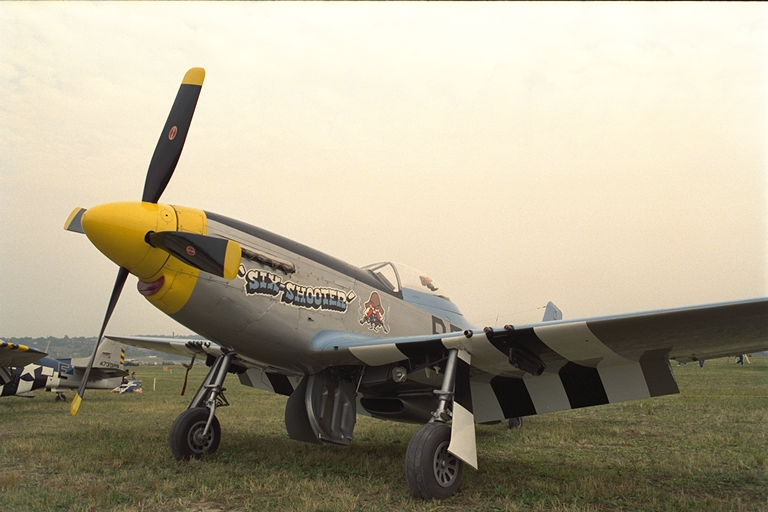
\includegraphics[width=0.5\textwidth]{imagenes/img9.png}
           \hfill
        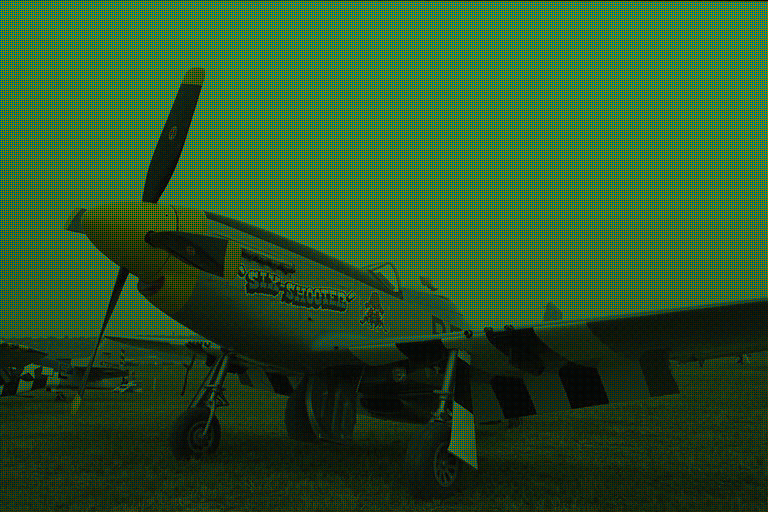
\includegraphics[width=0.5\textwidth]{imagenes/img9_bayer.png}   
        Imagen original y bayerizada
\end{figure}

\begin{figure}[h]
       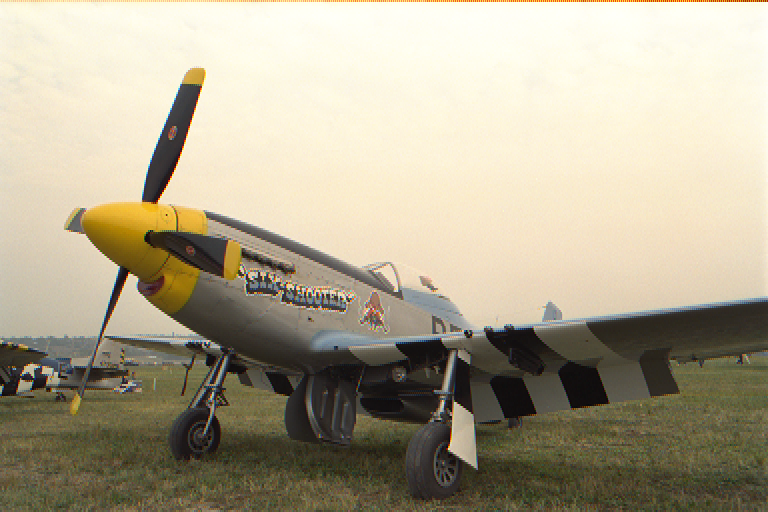
\includegraphics[width=0.5\textwidth]{imagenes/img9_demosicing_vecino.png}
           \hfill
        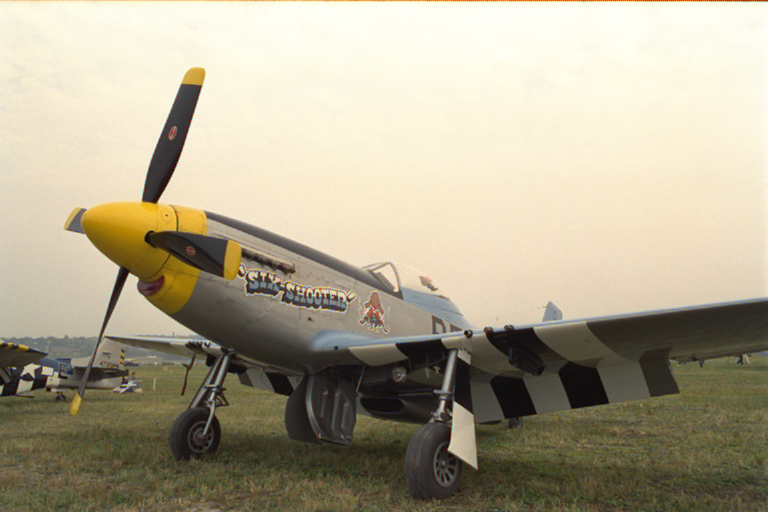
\includegraphics[width=0.5\textwidth]{imagenes/img9_demosicing_bilineal.png}
        Algoritmos de Vecinos e Interpolación Bilineal
\end{figure}


\begin{figure}[h]
       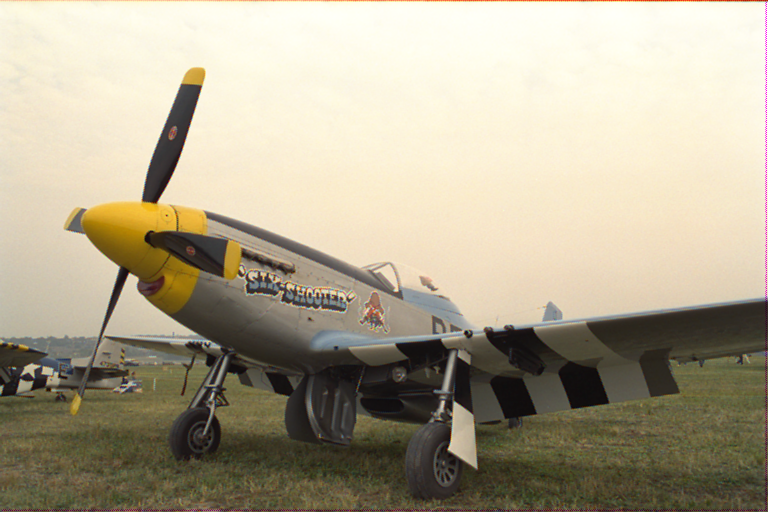
\includegraphics[width=0.5\textwidth]{imagenes/img9_demosicing_spline.png}
           \hfill
        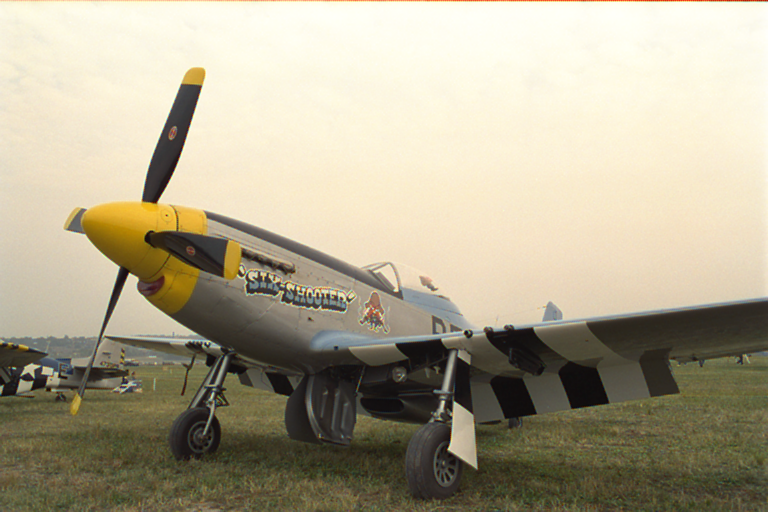
\includegraphics[width=0.5\textwidth]{imagenes/img9_demosicing_quality.png}
        Algoritmos de Interpolación Direccional y HighQuality
\end{figure}
\newpage

Como se puede observar, a simple vista pareciera que los 4 algoritmos dan un resultado bastante aceptable, pero mirando detalladamente y comparando entre sí se puede observar una gran diferencia entre ellos, principalmente en zonas borde y en la zona del texto del avión. Subjetivamente pareciera ser que la imagen más parecida a la original es la del HighQuality, seguida por la Interpolación Direccional, pero objetivamente en base a los resultados obtenidos al método PSNR se observa que el algoritmo de Interpolación Bilineal supera al Direccional, algo que llama bastante la atención y que indica que lo subjetivo se diferencia bastante de los objetivo. 

$$ 
\begin{bmatrix}
        algoritmo   &      PSNR     \\
       highquality    &   37.71  \\
       bilineal    &     35.34  \\
       directional    &      33.35    \\
       vecinos   &      30.49     \\
\end{bmatrix} 
$$
Yendo más a fondo aún en la cuestión y para mostrar el nivel de detalle que obtiene cada algoritmo, decidimos hacer zoom en la zona donde la imagen posee texto:

\begin{figure}
       
\includegraphics[width=0.5\textwidth]{imagenes/img9_demosicing_vecino_cropped.png}
        \caption{Vecinos}
\end{figure}

\begin{figure}
       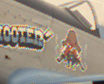
\includegraphics[width=0.5\textwidth]{imagenes/img9_demosicing_bilineal_cropped.png}
        \caption{Bilineal}
\end{figure}

\begin{figure}
       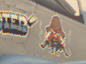
\includegraphics[width=0.5\textwidth]{imagenes/img9_demosicing_spline_cropped.png}
        \caption{Direccional}
\end{figure}

\begin{figure}
       
\includegraphics[width=0.5\textwidth]{imagenes/img9_demosicing_quality_cropped.png}
        \caption{Quality}
\end{figure}

Acá si se puede observar la nitidez y suavidad que presenta cada algoritmo, viéndose como mejora la calidad del texto para cada imagen y como va disminuyendo el ruido aumentando la refinación alrededor del mismo.

\newpage

\subsection{Imagen 12}

A continuación probaremos con una imagen provista por la cátedra para tener mas resultados sobre los cuales apoyarnos a la hora de sacar nuestras conclusiones. Obviaremos la imagen bayerizada ya que sólo
nos interesaba ver que sea correcta la bayerización y con lo ya hecho eso queda claro.

\begin{figure}[h]
\begin{center}
       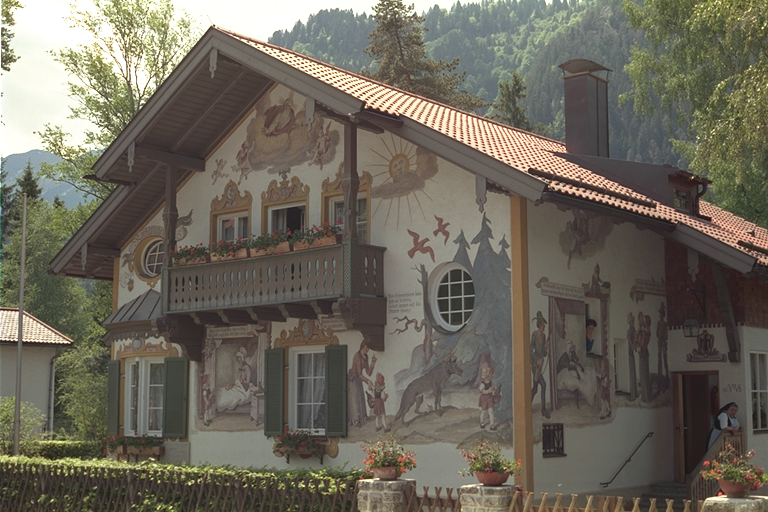
\includegraphics[scale=0.3]{imagenes/img12.png}
       \caption{Original }\label{fig:awesome_image1}
        \end{center}

\end{figure}

\begin{figure}[!ht]
\minipage{0.5\textwidth}
\begin{center}
    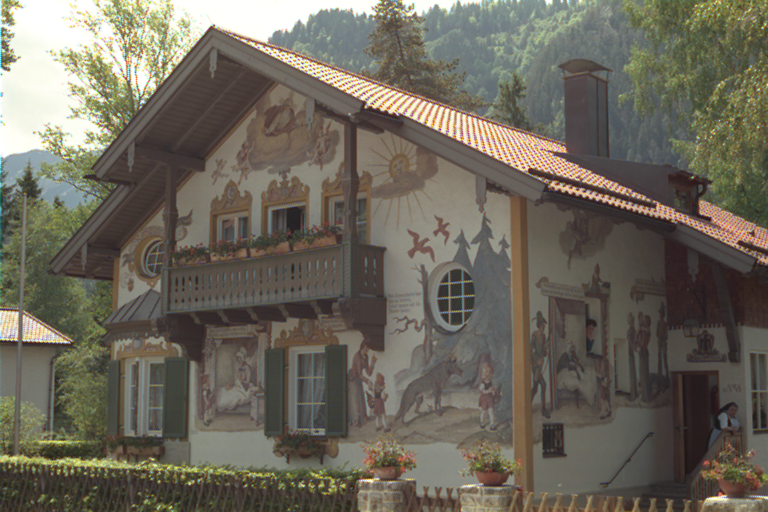
\includegraphics[scale=0.3]{imagenes/img12_demosicing_bilineal.png}
    \caption{Bilineal }
 \end{center}
\endminipage
\minipage{0.5\textwidth}
\begin{center}
    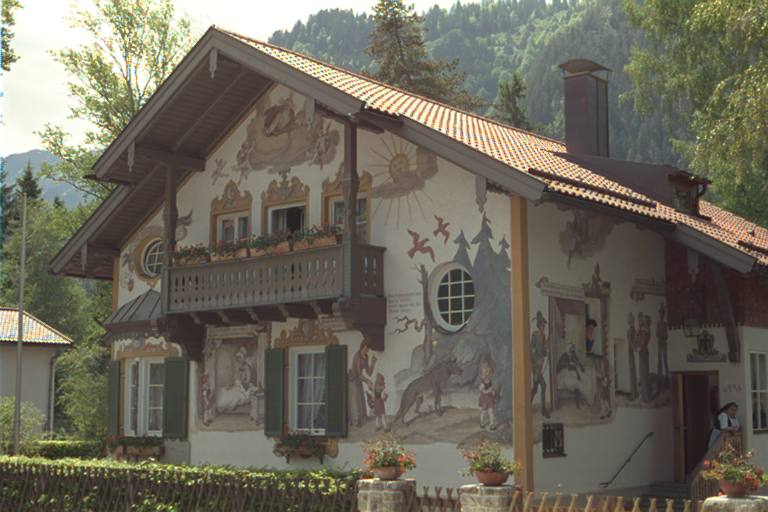
\includegraphics[scale=0.3]{imagenes/img12_demosicing_quality.png}
    \caption{High Quality}
        \end{center}
\endminipage\hfill
\end{figure}

\begin{figure}[h]
\minipage{0.5\textwidth}
\begin{center}
    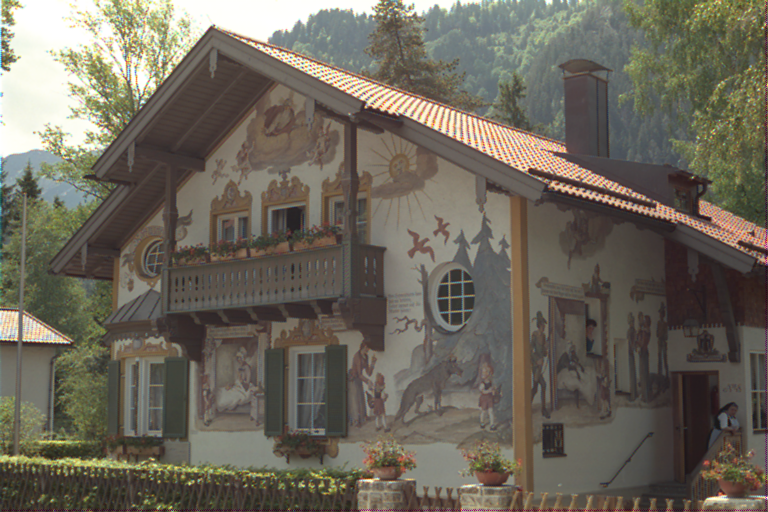
\includegraphics[scale=0.3]{imagenes/img12_demosicing_spline.png}
    \caption{Directional}
        \end{center}
\endminipage
\minipage{0.5\textwidth}
\begin{center}
    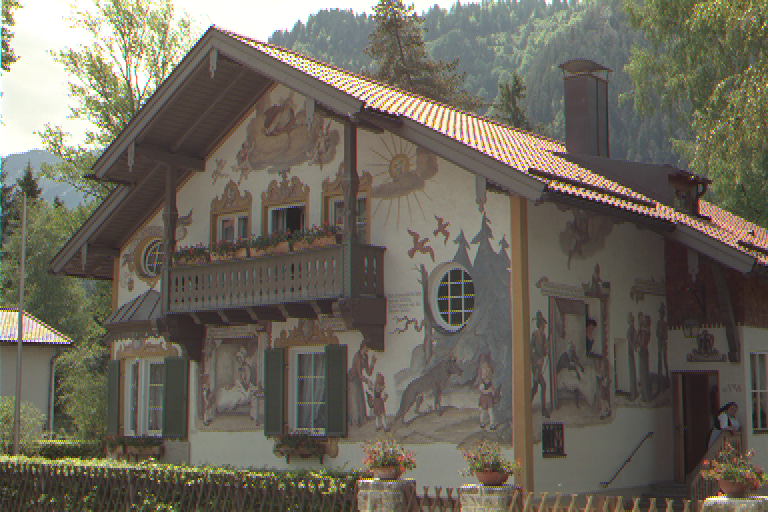
\includegraphics[scale=0.3]{imagenes/img12_demosicing_vecino.png}
    \caption{Vecinos}
 \end{center}
\endminipage
 
\end{figure}
\newpage

Subjetivamente highquality parece ser la mejor. Ya que se la ve bastante menos borrosa que las demás y con bordes mas nítidos, esto es facilmente apreciable en los dibujos que hay sobre la casa. A diferencia de vecinos que tiene bordes no sólo poco nítidos sino hasta claramente pixelados. Entre Directional y bilineal podemos notar que el primero, en los dibujos de la casa, es un poco más nitido que el segundo y parece tener un poco mas de calidad, también apreciable en los dibujos de la casa.

Veamos ahora a través del calculo del PSNR contra la imagen original como es el ranking.

$$ 
\begin{bmatrix}
           &      PSNR    \\
       quality    &   32.33   \\
       bilineal    &      30.27   \\
       directional    &      29.87    \\
       vecinos   &      25.45     \\
\end{bmatrix} 
$$

Objetivamente el peor y el mejor se mantienen, debido a que quality es el de mayor PSNR y vecinos el de menor. En estos valores también es apreciable la gran diferencia de resultados observada anteriormente, mientras que subjetivamente se podía notar una nítida y la otra directamente pixelada objetivamente el PSNR es 10 puntos mas grande en la quality. Lo que si cambia acá es la relación entre directional y bilineal, mientras que objetivamente el bilineal parecía ser mejor subjetivamente podemos ver que esto es al revés (aunque también por poca diferencia).

Como dato interesante vale aclarar que en el tejado de la casa podemos ver anomalías en todos los resultados, así como también en los arboles que están a la izquierda y por encima. Más adelante analizaremos bien porque es que sucede esto.


\newpage

\subsection{Calidad subjetiva}

En las secciones anteriores analizamos la calidad de las imágenes basándonos en los valores de los pixeles que resultaban después de aplicar los distintos algoritmos de demosaicing y la comparamos con la original pero no teníamos en cuenta las diferencias entre estas a la vista del ojo humano. Por esto último en esta sección mediremos la calidad subjetiva de las imágenes en base a los \textbf{artifacts} que se pueden encontrar en cada una de ellas.\\

\subsubsection{Moiré}


\begin{figure}[h]
\minipage{0.5\textwidth}
\begin{center}
       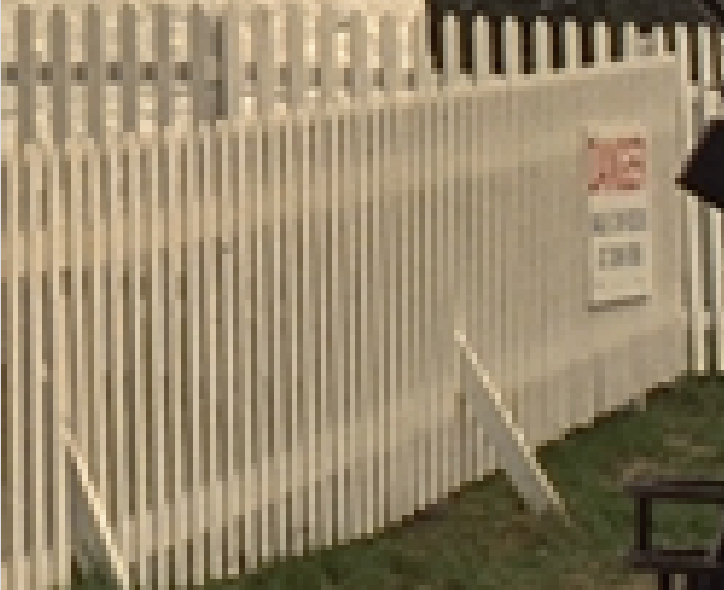
\includegraphics[width=0.5\textwidth]{imagenes/img8_moire_original.png}
        \caption{}
        \end{center}
\endminipage
\minipage{0.5\textwidth}
\begin{center}
       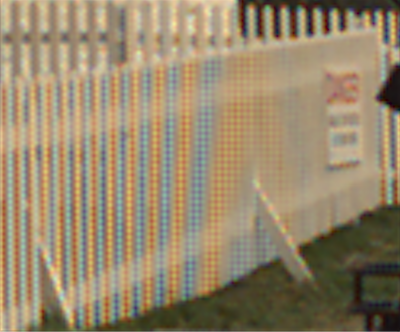
\includegraphics[width=0.5\textwidth]{imagenes/img8_moire.png}
        \caption{}
         \end{center}
\endminipage
\end{figure}

\subsubsection{False color}
\subsubsection{Zippering}
\subsubsection{Blur}
\subsubsection{Ringing}



\newpage
\section{Discusi\'on}


\newpage
\section{Conclusiones}

\subsection{Comparación de tiempos}

En esta sección presentaremos una comparativa entre los tiempos que tarda cada algoritmo a medida que aumenta el tamaño de la imagen. Para tal fin testamos cada algoritmo con imágenes cuadradas generadas aleatoriamente que van aumentando su tamaño, y creemos que es una forma correcta de comparar los tiempos ya que la complejidad de cada algoritmo es más independiente de la información que tenga la imagen que del tamaño debido a que las iteraciones depende directamente de este.

\begin{figure}[h]
       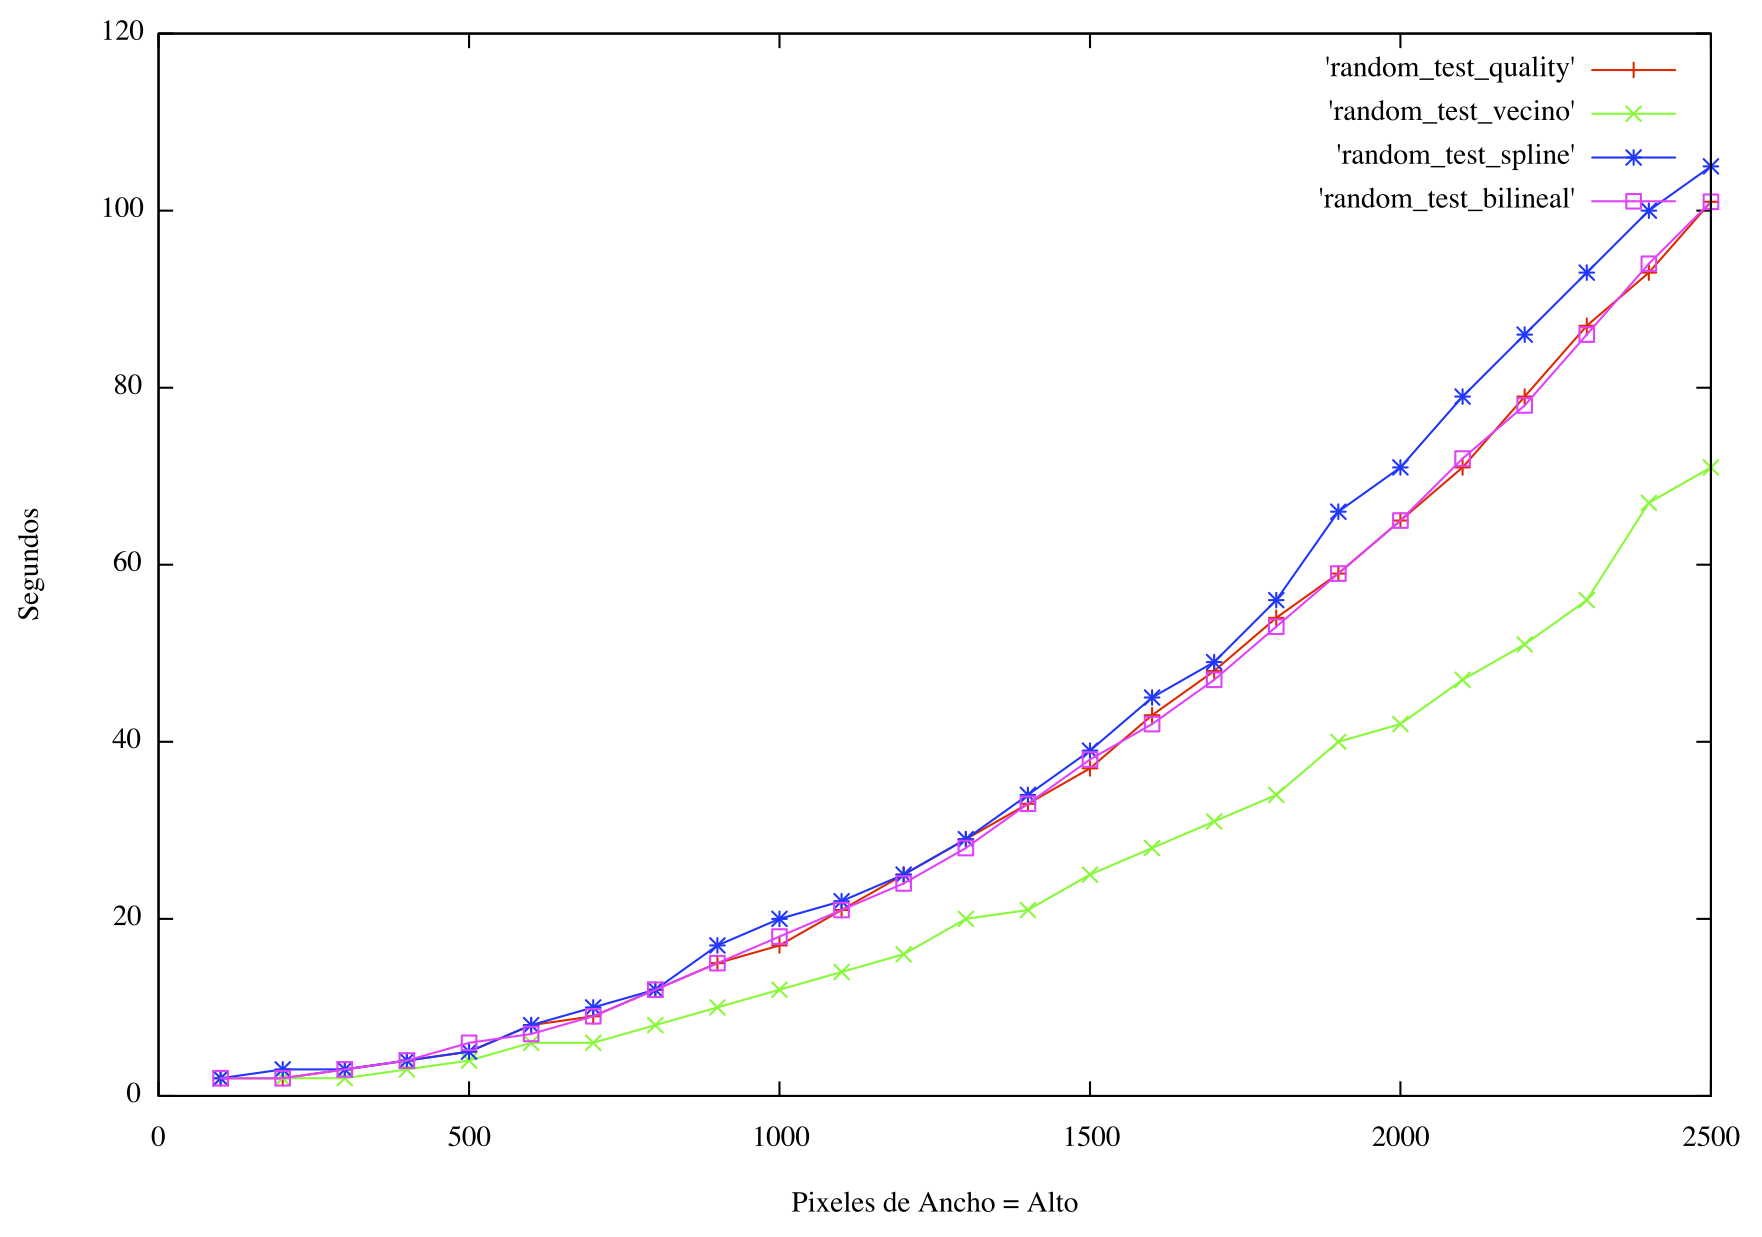
\includegraphics[width=1\textwidth]{imagenes/tiempo_algoritmos_random.png}
\end{figure}

Vecinos al ser el más simple, tiene sentido que haya tardado menos. Lo único que hace es recorrer la imagen y rellenar por cada color faltante de cada pixel, de, valga la redundancia, sus vecinos que captaron ese color en la bayerización. Bilineal en segundo puesto, ya que realiza un promedio y necesita ver más puntos. \\
Tanto Direccional y Quality, utilizan bilineal ya que no son algoritmos de aproximación de cero, si no de mejora. Por lo que ya tienen una cota inferior. Igualmente es notable que Quality siendo el mejor resultado, como venimos viendo en puntos anteriores y un detalle mejor en la próxima sección, también sea el de menor tiempo. Esto se debe a que tiene una cuenta parecida al bilineal pero en pocos píxeles, a diferencia de Direccional que resuelve un sistema de ecuaciones por cada fila y columna.\\
Igualmente no es poco notar que son bastantes lentos los algoritmos, y las pruebas si bien fueron con imágenes relativamente grandes, no alcanzan a las cámaras promedio que claramente no tardan 10 segundos en resolver la foto final. O existen optimizaciones que no llegamos a hacer o hay un mejor aprovechamiento del hardware, paralelismo, etc.
Como el algoritmo de HighQuality solamente procesa los verdes de la imagen, requerirá un $``poco"$ más de tiempo para imágenes que tengan una mayor calidad para ese color.




\subsection{Comparación de calidad}
En esta sección compararemos solo los verdes de las imágenes y veremos los resultados utilizando PSNR. Recordemos que este término, calcula nivel de ruido en una señal.

\begin{figure}[h]
       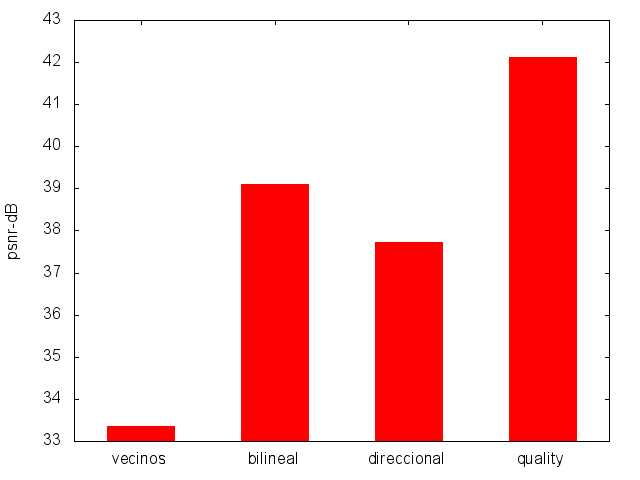
\includegraphics[scale=0.8]{imagenes/quality_performance.png}
       \caption{Img1}
\end{figure}

Como venimos viendo en otros ejemplos, img9, img12, y este, como era esperado, el vecinos es el que peor hizo, y quality fue el mejor. Sin embargo notemos que Spline si bien 
tendría que tener un valor mayor que bilineal ya que subjetivamente notamos mejora entre ellos, no lo tiene, es 
decir, el nivel de ruido es mayor en el direccional. Esto tiene sentido en la medida que el algoritmo direccional 
utiliza toda la fila y toda la columna para calcular el valor de las coordenadas $b_j$, $c_j$ y $d_j$ por lo que está 
sujeto a valores distintos al valor final, a diferencia de Bilineal que está sujeto a sus vecinos directos que es 
mucho más probable que tengan un valor más próximo. 


\subsection{Algoritmos}
En base a los algoritmos presentados, concluimos que a partir del tiempo de cómputo y resultados que ofrecen los mismos, siempre conviene optar por el algoritmo de HighQuality, ya que como se observa en las secciones anteriores, la calidad que ofrece es extremadamente buena y el tiempo que tarda es aceptable.
Otra cosa que nos llamo la atención fueron los resultados obtenidos por las dos interpolaciones bilineales y direccionales, ya que si bien en teoría la direccional debería obtener mejores resultados, estos solo se aprecian al mirarlos, es decir subjetivamente, ya que objetivamente el bilineal aproxima mejor los colores originales y obtiene un menor ruido en la señal del color verde.

\subsection{Bordes}
En caso de una imagen con cambios grandes en zonas pequeñas, todos los algoritmos tienden a fallar en esas zonas.
Esto se debe a que todos los algoritmos dependen fuertemente de los pixeles próximos cercanos, los cuales poseen valores muy distintos al valor a calcular. Esto es denominado borde.

Otro punto interesante es que si bien el algoritmo de High Quality funcionó mejor objetiva y subjetivamente para las imagenes que son fotografiías esto no fué así en el caso de la imagen $"$colores$"$. Pensamos que esto se debe a que este procedimiento fué especialmente pensado para fotografías, es decir imagenes con bordes mas suaves o sin tanta saturación de color de cada lado del borde. Y que es por esto que en este caso los resultados dieron casi lo contrario de todo el resto (vecinos fué el mejor en todo sentido).

\subsection{Otro uso}
Si bien el TP está apuntado a los algoritmos que corren en las cámaras de fotos, un uso útil puede ser el de compresión de imágenes, ya que bayerizando la imagen original reduce en un tercio su tamaño y en poco tiempo (menor aún en la práctica cuando lo usan las camáras digitales) se puede obtener la original, o al menos una aproximación bastante acertada de la misma.

\begin{thebibliography}{9}

\bibitem{Burden y Faires}
  $R. Burden y J.D.Faires, Analisis numerico, International Thomson Editors, 1998$

\bibitem{Ron Kimmel}
$Ron Kimmel. Demosaicing: image reconstruction from color ccd samples. IMAGE PRO-
CESSING, IEEE TRANSACTIONS ON, 1999.$

\end{thebibliography}

\newpage

\end{document}

